%%%%%%%%%%%%%%%%%%%%%%%%%%%%%%%%%%%%%%%%%%%%%%%%%%%%%%%%%%%%%%%%%%%%%%%%%%%%%
%%%%%%%%%%%%%%%%%%%%%%%%%%%%%%%%%%%%%%%%%%%%%%%%%%%%%%%%%%%%%%%%%%%%%%%%%%%%%
\chapter{RESULTS}

For both HMM and KF methods, all training points are taken in one continuous
sequence, and training is performed on a window of size $T$. Once training is
completed, predictions can then be made for the next $N$ days starting right
after the training window finished.

As we have seen, When we trained an HMM or KF over a continuous batch of time
series data, what we actually achieved is compressing that data into a shorter,
more compact form. In a sense the data shrinks and the resulting model gives us
a summary of what the data contains. Once this is completed and let us say we
wanted to re-generate data that was used to train the learner, theoretically
this should be possible - for instance for HMMs, starting with the initial
probabilities $\pi$, one can ``roll the dice'' based on $\pi$ and transition
matrix $A$, we can choose a transition, follow that to the next hidden state,
then we throw dice again which lets us follow a transition probability contained
in $A$, so on. This lets us to run a simulation of the data we used to train our
HMM. The real data could have contained 1000 points, however with a trained HMM,
all we really need is $\pi, A, \eta$. The rest is random number generation using
the HMM. For generating {\em future} values, we modified this method a little
further.


%%%%%%%%%%%%%%%%%%%%%%%%%%%%%%%%%%%%%%%%%%%%%%%%%%%%%%%%%%%%%%%%%%%%%%%%%%%%%

\section{Monte Carlo Simulation}

During our tests, we found that executing HMM or KF forward prediction ``once''
did not give optimal results. The reason for the bad performance was hypothized
to be related to pseudorandom number generation - our method, using HMM or KF
relies on pseudorandom number generation over gaussian and uniform
distributions. Especially when a prediction is performed for more than 5 days,
it was observed that the results would degenerate very rapidly. In order to
offset this issue, we decided that using Monte Carlo (MC) method could alleviate
these problems.

Monte Carlo method involves the use of pseudorandom numbers to generate results,
and each experiment is repeated many times to obtain better accuracy and
approximation. For HMM and KF pseudorandom number generation, we chose to follow
this method, then, in each case, the forward prediction which utilizes
pseudorandom number generation was repeated for over $500$ times. After each run
the predicted values of each iteration were summed and averaged for a final list
of predicted values. The iteration numbers were determined during training phase
where many different parameters were tested for optimal results. We observed
that the results improved considerably by this method.

For the generation of pseudorandom numbers, we employ Java
\textsuperscript{\textregistered} language's internal random number
generator. However, an important rule of MC simulation is that the experiments
need to be replicable - that is, each time the same experiment is executed, the
pseudorandom generation should be exactly the same as the previous run. The
default mode of Java pseudorandom number generation takes the current time as
its seed. This would give us different random number for each run. We had to
modify this by setting the seed ourselves manually. A hex value large enough
such as \verb!0x5DAE6EE6DL!  yielded good results.

%%%%%%%%%%%%%%%%%%%%%%%%%%%%%%%%%%%%%%%%%%%%%%%%%%%%%%%%%%%%%%%%%%%%%%%%%%%%%
%%%%%%%%%%%%%%%%%%%%%%%%%%%%%%%%%%%%%%%%%%%%%%%%%%%%%%%%%%%%%%%%%%%%%%%%%%%%%

\section{Results}

For our testing we used ISE-100 Index historical data between dates 30/10/1987
and 29/1/2008, for DJI between dates 02/02/1970 and 02/02/2007. Two thirds of
the data was used for training (to adjust model parameters) then the rest of the
data was used for testing final results.

We picked single Gaussian as our HMM's emission distribution and determined 7 to
be the number of hidden states. All HMM, KF and KMM methods used a single
dimension to model their input data. Important parameters used for all methods
are presented below:

\begin{table}[h]
\caption{Parameters}
\vspace{0.3cm}
\begin{tabular}{|l|l|l|}
\hline 
\textbf{Method} & \textbf{Parameter} & \textbf{Value} \\
\hline 
HMM & \# of hidden states  & 7 \\
\hline
ANN - ISE & \# of inputs & 1700 \\
\hline
ANN - DJI & \# of inputs & 3000 \\
\hline
ANN & \# of output & 1 \\
\hline
ANN & \# of Neurons in Hidden Layer & 30 \\
\hline
Polynomial & Degree & 10 \\
\hline
ANN - ISE and DJI & Size of Training Window & 300 \\
\hline
All (except ANN) - ISE & Size of Training Window & 1700 \\
\hline
All (except ANN) - DJI & Size of Training Window & 3000 \\
\hline
\end{tabular}
\end{table}


Kalman/HMM/KMM testing involved a runner program that was able to divide the
data into appropiate pieces, forming one test run, executing it and collecting
the results. In order to increase the number of test runs, we decided to form a
``shifting window'' in the data, running HMM/Kalman/KMM training and prediction
on this window. The training window was shifted 30 times for each run. The
runner starts with a section of data $W$ wide, trains the model, predicts the
next 1,5 and 10 days and compares the results against actual stock price
data. While comparing predicted vs. actual data, the runner program collects
various metrics. A short description of these metrics can be found below;

\subsection{Metrics}

\textbf{MSE Ror}: This metric's long name is mean square error for rate of
returns. In general we can say in our application we collect three types of
metrics: Prediction error on rate of returns, prediction error on absolute
prices and hit rates for increase and decrease predictions. {\em MSE Ror} falls
in the ``rate of returns'' category.  The formula for mse ror is below; $R_i$ is
real rate of returns, $S_i$ is the real stock price, $X_i$ is estimates for rate
of returns or prices on day $i$ and $N$ is the number of predictions, MSE Ror
is:
\begin{eqnarray}
\sqrt{\frac{\sum_i (R_i - X_i)^2}{N}}. 
\end{eqnarray}
\textbf{MAE Ror}: The long name for this metric is ``mean absolute error for
rate of returns''. It calculates the absolute error between predicted rate of
returns and real values. The formula for it is 
\begin{eqnarray}
\frac{\sum_i (|R_i - X_i|)}{N}
\end{eqnarray}
\textbf{MSE Price} statistic is very similar to MSE Ror except that instead of
rate of returns we are using the stock prices themselves. This metric is
formulized as 
\begin{eqnarray}
\sqrt{\frac{\sum_i (S_i - X_i)^2}{N}}
\end{eqnarray}
\textbf{MAE Price} is similar to MAE Ror except that instead of rate of returns
we are using the stock prices themselves which is formulized as
\begin{eqnarray}
\frac{\sum_i (|S_i - X_i|)}{N}
\end{eqnarray}
\textbf{HR} whose long name is ``hit rate'' calculates the number of times
(days) the model succeeded in making a correct increase or decrease prediction
for stock price data. This metric does not look at actual amount of increase in
price, it simply looks at the rate of returns metric and compares the ``signs''
of predicted and actual values. Since rate of returns inherently reveal whether
stock price increased or decreased, the comparison of signs suffices for hit
rate calculations. {\em HR+} captures the number of times an increase was
predicted correctly, {\em HR-} captures the number of times a decrease was
predicted correctly. {\em HR} is a sum of HR+ and HR-.

\subsection{Plots}

To produce the plots seen in \ref{1day1} and \ref{1day2} of ``one day ahead''
predictions, we used a shifting training window $W$ of size $1700$. HMM, KF and
KMM were trained using data points $t,...,t+W$ and using the trained model, we
generated a prediction for the next day, $t+W+1$. Then the training window is
shifted to the right by one day and the same procedure is repeated. This
procedure was performed for 30 days. The predictions, along with the actual
index price for each day are plotted side by side in the same graph. This graph
was inspired by Hassan and Nath \cite{hassan} (covered in Section
\ref{prevwork}) who used it to display their method's results. The comparison of
our graph and theirs can give a good sense of both methods in terms of
prediction success.

\begin{figure}[!hbp]
\center{
  \scalebox{0.35}{
  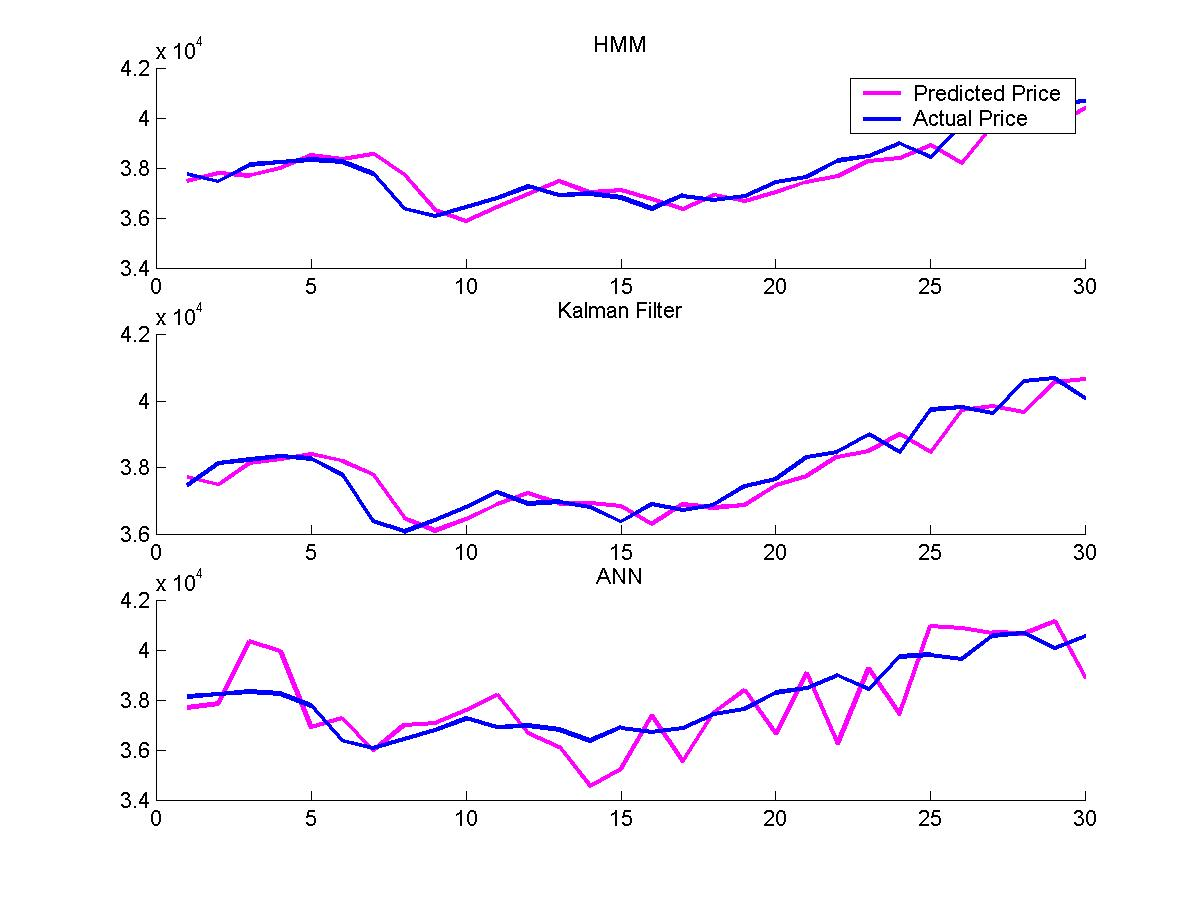
\includegraphics{./results/1-day-imkb-1.jpg}
  }
}

\caption{\label{1day1} One Day ISE-100 Predictions Using HMM, KF and ANN}
\vspace{0.6cm}
\end{figure}

\begin{figure}[!hbp]
\center{
  \scalebox{0.35}{
  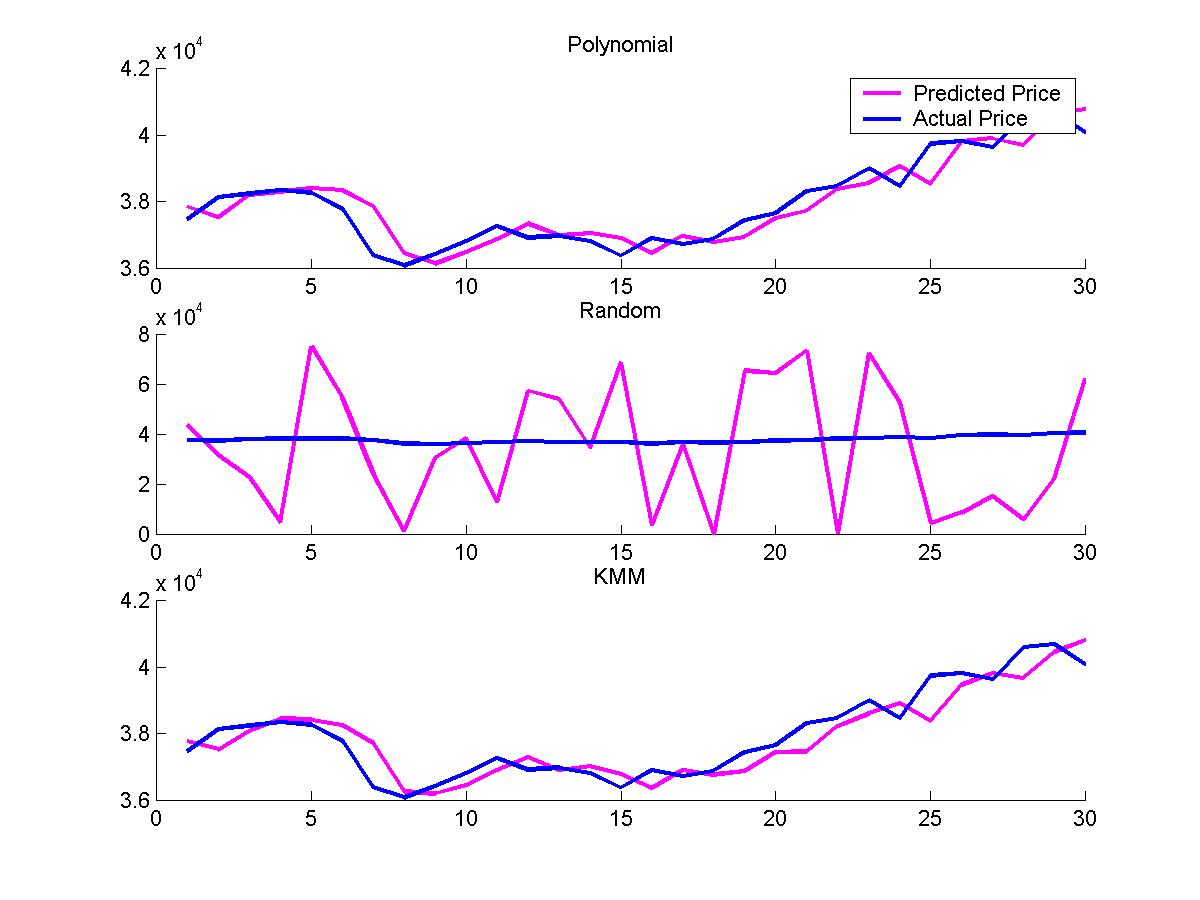
\includegraphics{./results/1-day-imkb-2.jpg}
  }
}
\caption{\label{1day2}One Day ISE-100 Predictions Using polynomial, random and KMM}
\vspace{0.6cm}
\end{figure}


\begin{figure}[!hbp]
\center{
  \scalebox{0.65}{
  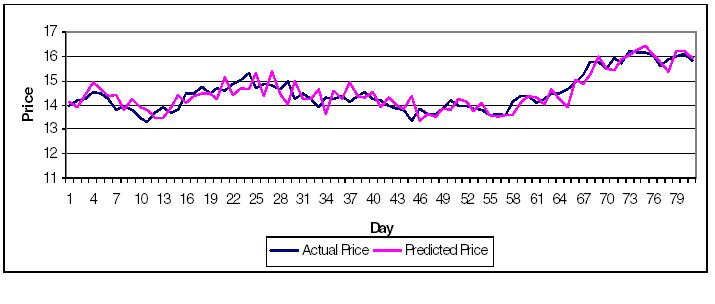
\includegraphics{./results/hasannath.JPG}
  }
}
\caption{\label{1day5}One Day Predictions Using HMM method by Hassan \& Nath \cite{hassan}}
\label{1dayhassan}
\vspace{0.6cm}
\end{figure}


\subsection{Conclusion}

\begin{table}[h]
\caption{\label{table1}ISE Prediction - 1 day}
\vspace{0.3cm}
\begin{tabular}{|l|l|l|l|l|l|l|}
\hline
 &                  HMM &       Kalman &   Random &        ANN &     Polynomial &    KMM\\
\hline
   MSE Ror &      0.011 &      0.011 &      0.049 & 0.01154460 &      0.015 &      0.012\\
\hline
 MSE Price &    114.715 &     36.446 &   2176.878 & 1.24473817 &    518.535 &    156.740\\
\hline
   MAE ROR &      0.011 &      0.011 &      0.049 & 0.01154460 &      0.020 &      0.012\\
\hline
 MAE Price &    114.715 &     36.446 &   2176.878 & 1.24473817 &    518.535 &    156.740\\
\hline
        HR &      0.567 &      0.700 &      0.467 & 0.54838710 &      0.581 &      0.600\\
\hline
        H+ &      0.333 &      0.467 &      0.267 & 0.32258065 &      0.581 &      0.400\\
\hline
        H- &      0.233 &      0.233 &      0.200 & 0.22580645 &      0.000 &      0.200\\
\hline
\end{tabular}
\end{table}

As ``one day ahead'' predictions (seen in Table \ref{table1}) show , HMM, KF and
KMM methods offer results that are better than random and polynomial based
predictions. Kalman filters offer the best prediction in hit rate categories,
but the differences are especially obvious in absolute price categories. The
only contender here was the ANN method, it was able to surpass KF prediction in
terms of {\em MAE} and {\em MSE} metrics. Also, KF predictions in these
categories are almost one third of HMMs. Most promising result was the {\em HR}
result, for KF at 70\%. ANN and polynomial {\rm HR} results were better than
HMM. The winner here are both ANN and KF methods. For trading purposes, I would
use KF because of its success at hit rate metrics.

\begin{table}[h]
\caption{\label{table2}ISE Prediction - 5 days}
\vspace{0.3cm}
\begin{tabular}{|l|l|l|l|l|l|l|}
\hline
 &                  HMM &       Kalman &   Random &        ANN &     Polynomial &    KMM\\
\hline
   MSE Ror &      0.007 &      0.007 &      0.027 & 0.00656345 &      0.007 &      0.007\\
\hline
 MSE Price &    382.314 &    375.512 &   1727.495 & 273.23645268 &    428.181 &    414.425\\
\hline
   MAE ROR &      0.012 &      0.012 &      0.053 & 0.01199135 &      0.015 &      0.013\\
\hline
 MAE Price &    690.210 &    690.491 &   3415.059 & 444.12065452 &    827.508 &    765.393\\
\hline
        HR &      0.527 &      0.493 &      0.440 & 0.58709677 &      0.490 &      0.467\\
\hline
        H+ &      0.273 &      0.240 &      0.240 & 0.28387097 &      0.490 &      0.213\\
\hline
        H- &      0.253 &      0.253 &      0.200 & 0.30322581 &      0.000 &      0.253\\
\hline
\end{tabular}
\end{table}

As the number of days being predicted increases (seen in Table \ref{table2}), we
notice two things: The error rates in terms of absolute prices start increasing
and second, in terms of {\em HR} metric, the difference between HMM and KF and
their closest contender polynomial method decreases as well. In fact, all
methods start approaching random prediction which in the long run must approach
\%50 success rate. In terms of {\em MAE} metric, ANN method was the top
performer, closely follwed by HMM, KF and KMM methods. One surprise here was
ANN's {\em HR} metric, it was at \%58 which for 5 day prediction is still a very
good result. However we did not witness the same level of success for DJI 5-day
prediction, hence we contributed this success to being ``lucky'', perhaps due to
random number generation outputting just the right values, or to precision
somehow working in the method's favor. The top performer in terms of {\em MSE}
results is again ANN at around \%0.006, so the method's overall performance is
still very good. The difference between the top performers and random prediction
is almost tenfold. Random prediction is doing very badly, which, of course it
should.

\begin{table}[h]
\caption{\label{table3}ISE Prediction - 10 days}
\vspace{0.3cm}
\begin{tabular}{|l|l|l|l|l|l|l|}
\hline
 &                  HMM &       Kalman &   Random &        ANN &     Polynomial &    KMM\\
\hline
   MSE Ror &      0.005 &      0.005 &      0.019 & 0.00514647 &      0.005 &      0.005\\
\hline
 MSE Price &    407.231 &    424.893 &   1514.800 & 229.06783797 &    456.783 &    437.967\\
\hline
   MAE ROR &      0.013 &      0.013 &      0.053 & 0.01301490 &      0.014 &      0.014\\
\hline
 MAE Price &   1064.323 &   1107.195 &   4116.571 & 547.09327032 &   1239.209 &   1146.643\\
\hline
        HR &      0.500 &      0.497 &      0.437 & 0.52580645 &      0.510 &      0.483\\
\hline
        H+ &      0.270 &      0.240 &      0.223 & 0.25806452 &      0.506 &      0.230\\
\hline
        H- &      0.230 &      0.257 &      0.213 & 0.26774194 &      0.003 &      0.253\\
\hline
\end{tabular}
\end{table}

For 10 day predictions (seen in Table \ref{table3}), we see that all methods
with the exception of random prediction started approaching the same performance
numbers in terms of {\em HR}. This is an indication that prediction 10 days
ahead is a very hard task, and also, that each method is losing its
advantage. Here, again, polynomial method was consistent in its success, however
it also has a problem that its {\em H-} metric which is at a nearly zero. In
comparison its {\em H+} result is at ~\%50, this means the method has a
bias toward increases. This bias would cause problems if one wanted to use this
method for any form of trading activity.

The closeness of the results can be witnessed not only for {\em HR} metric, but
also for absolute price and {\em HR} statistics. ANN method reported the best
prediction in terms of absolute stock prices.

It is clear looking at all {\em HR} numbers that for 10 days, we are at a level
where random prediction is as good as any other method. Since the probability of
guessing an increase and decrease are both ~$0.25$ (in total $0.5$) in the long
run, we can see all methods are in the neighborhood of those numbers, in other
words, predicting the increase and decrease 10 days ahead is as good as flipping
a coin.

\begin{table}[h]
\caption{\label{table4}Dow Jones Prediction - 1 day}
\vspace{0.3cm}
\begin{tabular}{|l|l|l|l|l|l|l|}
\hline
 &                  HMM &       Kalman &   Random &        ANN &     Polynomial &    KMM\\
\hline
   MSE Ror &      0.005 &      0.005 &      0.058 & 0.00580727 &      0.009 &      0.005\\
\hline
 MSE Price &     10.305 &      3.694 &    654.055 & 0.08456436 &     57.121 &     18.566\\
\hline
   MAE ROR &      0.005 &      0.005 &      0.058 & 0.00580727 &      0.011 &      0.005\\
\hline
 MAE Price &     10.305 &      3.694 &    654.055 & 0.08456436 &     57.121 &     18.566\\
\hline
        HR &      0.600 &      0.633 &      0.500 & 0.57142857 &      0.548 &      0.600\\
\hline
        H+ &      0.367 &      0.367 &      0.233 & 0.33333333 &      0.290 &      0.367\\
\hline
        H- &      0.233 &      0.267 &      0.267 & 0.23809524 &      0.258 &      0.233\\
\hline
\end{tabular}
\end{table}

For ``one day ahead'' predictions using DJI values (seen in Table \ref{table4}),
we see similar performances as we saw with ISE-100 predictions. This actually is
a relief because it proves that financial time series data behaves in similar
ways to ISE time series values, and the trends are the same no matter which
stock, index or country the prices are based on. More similarities can be seen
in all metrics - for example {\em MSE Ror} difference between HMM/KF/KMM and
polynomial prediction are still within 40\%, {\em HR} success of KF method is
the best, closely followed by ANN, HMM and KMM and then polynomial
methods. There is almost a tenfold difference between {\em MSE Ror} for KF and
random prediction. In terms of rate of return prediction, HMM/KF/KMM reported
the best results even though in terms of absolute prices, ANN still performed
better than all of the other methods. 

\begin{table}[h]
\caption{\label{table5}Dow Jones Prediction - 5 days}
\vspace{0.3cm}
\begin{tabular}{|l|l|l|l|l|l|l|}
\hline
 &                  HMM &       Kalman &   Random &        ANN &     Polynomial &    KMM\\
\hline
   MSE Ror &      0.003 &      0.003 &      0.025 & 0.00247295 &      0.003 &      0.003\\
\hline
 MSE Price &     45.048 &     43.990 &    403.774 & 21.49305772 &     51.288 &     47.909\\
\hline
   MAE ROR &      0.005 &      0.005 &      0.050 & 0.00449691 &      0.005 &      0.005\\
\hline
 MAE Price &     83.589 &     82.309 &    797.036 & 35.36699410 &    103.298 &     89.661\\
\hline
        HR &      0.460 &      0.553 &      0.473 & 0.51428571 &      0.587 &      0.460\\
\hline
        H+ &      0.320 &      0.347 &      0.307 & 0.30476190 &      0.329 &      0.293\\
\hline
        H- &      0.140 &      0.207 &      0.167 & 0.20952381 &      0.258 &      0.167\\
\hline
\end{tabular}
\end{table}

And just as was the case with ISE predictions, HMM/KF and polynomial results
start approaching eachother as number of predicted days start to increase (seen
in Table \ref{table5}). However, in terms of DJI prediction, this approach
happen much earlier (at 5 days) than was the case with ISE predictions. With ISE
prediction, it was not until 10 days that the results came close to each other. 

\begin{table}[h]
\caption{\label{table6}Dow Jones Prediction - 10 days}
\vspace{0.3cm}
\begin{tabular}{|l|l|l|l|l|l|l|}
\hline
 &                  HMM &       Kalman &   Random &        ANN &     Polynomial &    KMM\\
\hline
   MSE Ror &      0.002 &      0.002 &      0.018 & 0.00187652 &      0.002 &      0.002\\
\hline
 MSE Price &     41.802 &     43.171 &    376.496 & 18.27777881 &     44.407 &     41.473\\
\hline
h   MAE ROR &      0.005 &      0.005 &      0.051 & 0.00477930 &      0.005 &      0.005\\
\hline
 MAE Price &    111.533 &    117.051 &   1012.789 & 44.48823690 &    123.517 &    110.753\\
\hline
        HR &      0.510 &      0.557 &      0.537 & 0.47619048 &      0.484 &      0.527\\
\hline
        H+ &      0.320 &      0.283 &      0.287 & 0.28095238 &      0.235 &      0.290\\
\hline
        H- &      0.190 &      0.273 &      0.250 & 0.19523810 &      0.248 &      0.237\\
\hline
\end{tabular}
\end{table}


As one can see from the data tables \ref{table1},\ref{table2},\ref{table3},
\ref{table4},\ref{table5} and \ref{table6} all methods were able to consistenly
outperform random number based prediction. We expected to see those results. In
respect to {\em MSE} and {\em MAE} metrics, ANN, HMM, KF and KMM methods are
found to be superior to other methods. For ``one day ahead'' prediction, KF
based prediction was best in terms of {\em HR} metric. The downside with
polynomial fitting was its {\em H-} metric always reported values close to zero,
which means this method was not able to guess market decreases meaning it is
biased. HMM, KF, KMM and ANN methods all have a healthy allocation between {\em
  H+} and {\em H-} values.


The ``one day ahead'' plots make the success of the guesses quite visible as
well. One point that needs mentioning here is that it could be misleading to
compare our graph directly with Hassan and Nath's, because they have
consistently used the four values mentioned in order to ``find'' an HMM whereas
we used one single HMM to ``generate'' a rate of return which we use to multiply
with the last days' ``known'' price.

In terms of trading, various strategies can be devised in order to maximize
return on investment. A simple trading strategy that takes a single stock or
index as a basis for trade could decide to ``buy'' a stock if it predicts
increase, or a``sell'' if it predicts a decrease for the next day. In case of
``buy'' and ``sell'' sequence, the difference would be profit. In case of
``sell'' and ``buy'' sequence. In other words we could still make money, by
extending this strategy in order to make money from ``decreases'' in the
market. Most markets offer a trading activity called ``short selling'' which
allows a trader to sell a security he does not own, in hope of repurchasing them
at a lower price. If I know the price of a security decrease to \$100 tomorrow,
and the price is \$120 today, I can shortsell at \$120, with a commitment to buy
the actual stock tomorrow. Then if the price falls, I will be buying at a lower
price selling it higher, pocketing the difference as profit.

Overall we can conclude HMM/KF/KMM methods performed reasonably well and they
can be used as a basis for a trading system.
